\documentclass[
  print,
  table,
  nolof,
  nolot,
  nocover,
  oneside
]{fithesis3}

\usepackage[resetfonts]{cmap}
\usepackage[T1,T2A]{fontenc}
\usepackage[
  main = english
]{babel}

\usepackage{paratype}
\def\textrussian#1{{\usefont{T2A}{PTSerif-TLF}{m}{rm}#1}}

\usepackage{xcolor}
\definecolor{bluekeywords}{rgb}{0,0,1}
\definecolor{greencomments}{rgb}{0,0.5,0}
\definecolor{redstrings}{rgb}{0.64,0.08,0.08}
\definecolor{xmlcomments}{rgb}{0.5,0.5,0.5}
\definecolor{light-gray}{gray}{0.95}
\definecolor{types}{rgb}{0.17,0.57,0.68}

\usepackage{listings}
\lstset{language=[Sharp]C,
  captionpos=b,
  showspaces=false,
  showtabs=false,
  breaklines=true,
  showstringspaces=false,
  breakatwhitespace=true,
  escapeinside={(*@}{@*)},
  commentstyle=\color{greencomments},
  morekeywords={partial, var, value, get, set, from, where, select},
  keywordstyle=\color{bluekeywords},
  stringstyle=\color{redstrings},
  backgroundcolor=\color{light-gray},
  basicstyle=\ttfamily\small
}

\usepackage{paralist}
\usepackage{amsmath}
\usepackage{amsthm}
\usepackage{amsfonts}
\usepackage{url}
\usepackage{markdown}

\usepackage{filecontents}
\usepackage{pgfplots}
\pgfplotsset{compat=1.14}

\usepackage[normalem]{ulem}
\usepackage{float}

\usepackage{fourier}
\DeclareMathAlphabet{\mathcal}{OMS}{cmsy}{m}{n}
\SetMathAlphabet{\mathcal}{bold}{OMS}{cmsy}{b}{n}

\newcommand\tab[1][1cm]{\hspace*{#1}}

\begin{filecontents}{100tests.dat}
1 823 955 765 1031 696
2 4102 4193 3802 4715 3690
3 4100 4206 4019 4379 3978
\end{filecontents}

\begin{filecontents}{500tests.dat}
1 925 957 886 1072 851
2 4351 4384 4291 4457 4240
3 5320 5410 5214 5526 5089
\end{filecontents}

\begin{filecontents}{1000tests.dat}
1 1055 1186 1032 1236 1005
2 4922 5364 4828 5613 4748
3 6927 7146 6809 7682 6691
\end{filecontents}

\pgfplotsset{
    box plot/.style={
        /pgfplots/.cd,
        black,
        only marks,
        mark=-,
        mark size=1em,
        /pgfplots/error bars/.cd,
        y dir=plus,
        y explicit,
    },
    box plot box/.style={
        /pgfplots/error bars/draw error bar/.code 2 args={%
            \draw  ##1 -- ++(1em,0pt) |- ##2 -- ++(-1em,0pt) |- ##1 -- cycle;
        },
        /pgfplots/table/.cd,
        y index=2,
        y error expr={\thisrowno{3}-\thisrowno{2}},
        /pgfplots/box plot
    },
    box plot top whisker/.style={
        /pgfplots/error bars/draw error bar/.code 2 args={%
            \pgfkeysgetvalue{/pgfplots/error bars/error mark}%
            {\pgfplotserrorbarsmark}%
            \pgfkeysgetvalue{/pgfplots/error bars/error mark options}%
            {\pgfplotserrorbarsmarkopts}%
            \path ##1 -- ##2;
        },
        /pgfplots/table/.cd,
        y index=4,
        y error expr={\thisrowno{2}-\thisrowno{4}},
        /pgfplots/box plot
    },
    box plot bottom whisker/.style={
        /pgfplots/error bars/draw error bar/.code 2 args={%
            \pgfkeysgetvalue{/pgfplots/error bars/error mark}%
            {\pgfplotserrorbarsmark}%
            \pgfkeysgetvalue{/pgfplots/error bars/error mark options}%
            {\pgfplotserrorbarsmarkopts}%
            \path ##1 -- ##2;
        },
        /pgfplots/table/.cd,
        y index=5,
        y error expr={\thisrowno{3}-\thisrowno{5}},
        /pgfplots/box plot
    },
    box plot median/.style={
        /pgfplots/box plot
    }
}


\thesissetup{
  date          = {2017/12/01},
  university    = {mu},
  faculty       = {fi},
  type          = {bc},
  author        = {Dávid Urbančok},
  gender        = {m},
  advisor       = {Bruno Rossi{,} PhD},
  title         = {Working with Complex SQL Queries in Unit Tests},
  TeXtitle      = {Working with Complex SQL Queries in Unit Tests},
  keywords      = {Kentico, unit testing, integration testing, Info object, InfoProvider object, DataSource, NUnit framework, performance},
  TeXkeywords   = {Kentico, unit testing, integration testing, Info object, InfoProvider object, DataSource, NUnit framework, performance},
  bib           = sources.bib,
}

\thesislong{abstract}{
This thesis is aimed at analyzing and extending the existing support of faking objects in Kentico's automated unit tests and its insufficiency when performing in-memory join operations on these objects.

After the analysis, a prototype solution that allows the joining to be performed in the memory is proposed and implemented.

This solution will allow rewriting some integration tests to unit tests in order to eliminate the need to run these tests against a database. This will increase performance and decrease the running time of the automated tests in Kentico's continuous integration tool.

Lastly, performance measurements are made to determine the time gain of this prototype and an estimation is calculated how much computing time is saved.
}

\thesislong{thanks}{
I would like to thank my supervisor, Bruno Rossi, PhD, who has helped me a lot with various invaluable inputs into this thesis. I would also like to extend my gratitude to Mgr. Michal Pietrik for countless hours of consultation and help with the implementation.
}

\begin{document}

% =============================================================================================
% INTRODUCTION ================================================================================
% =============================================================================================
\chapter{Introduction}

In today's world, testing is not just a complement to the development phase of a software product but its full and inseparable part. Undoubtedly, some parts of the testing process need still be done manually, others can be fully automated. Sometimes the automated tests run periodically in CI\footnote{Continuous integration} to ensure the maximum quality and responsiveness to changes in code.

Automated testing is a cheap way of maintaining the overall quality of a software. Automated tests can not only discover bugs but also make sure that any kind of refactoring does not break the intended functionality of the code.

Whether a company uses TDD\footnote{Test-driven development} or integrate automated tests in their software in other ways, these tests are necessary for any successful long-term project. Without automated tests, the software is prone to bugs without repeated manual re-testing.

It is not always possible to use real objects for the testing and that is why \textit{fake} or \textit{mock} objects are used. These terms are sometimes used as synonyms, some approaches, on the other hand, consider them different.

Different types of tests exist as a way of testing on more levels and different ranges of the SUT\footnote{System under test}. From the smallest - \textit{unit} tests that test the functionality of a single method or unit, through \textit{integration} tests testing different parts correctly working together, all the way to \textit{system} tests that test the system as a whole. This thesis focuses mainly on \textit{unit} and \textit{integration} tests.

While it is easy in theory to differentiate between the types of tests, in real life, it might be more difficult to draw the line. Sometimes a \textit{unit} test testing a single method is not enough as a result of current implementation or design that might require, for example, a database for this method to function correctly. This is only one example of a situation where usually \textit{unit} tests are used but are not enough due to incomplete isolation of this test from external dependencies.

The aim of this thesis is to analyze faking objects in Kentico CMS\footnote{https://en.wikipedia.org/wiki/Kentico\_CMS} and its insufficiencies when it comes to performing complex SQL operations on Kentico's objects, namely the \textit{JOIN} operation.

The thesis is divided into six chapters, the first of which introduces the reader the context and briefly explains the problem this thesis addresses.

In the second chapter, Kentico's back-end that consists of \textit{Info} and \textit{InfoProvider} objects is described with a sample implementation that allows for an easier understanding of the functionality of these objects.

The third chapter describes \textit{DataQuery} which is Kentico's object-oriented abstraction of the database query for reading data. The chapter further discusses its functionality and current drawbacks of using the more complex \textit{JOIN} operation in the memory.

The fourth chapter outlines automated testing, its importance and the types of tests discussed in this thesis. This chapter also provides a few examples of how to mimic real objects in tests using \textit{fakes} or \textit{mocks}.

The fifth chapter discusses automated testing in Kentico, what types of tests are used in Kentico and also gives a brief description of \textit{NUnit}\footnote{https://github.com/nunit/nunit} framework that is used for automated testing in Kentico.

The last, sixth, chapter describes the solution in the form of a new layer of abstraction that is implemented to allow in-memory \textit{JOIN} operation on objects using \textit{LINQ}\footnote{.NET Language-Integrated Query}. This chapter also presents the performance improvement on tests and discusses further extensions or alternative solutions.



% =============================================================================================
% KENTICO STRUCTURE ===========================================================================
% =============================================================================================
\chapter{Kentico's CMS structure}

Kentico is a content management system (CMS) developed by Kentico Software located in Brno, Czech Republic. CMS is a software system that provides website authoring, collaboration, and administration tools designed to allow users with little knowledge of web programming languages or markup languages to create and manage website content\parencite{cms}.

Kentico's functionality covers five areas: content management, e-commerce, social networking, intranet, and online marketing. It utilizes \textit{ASP.NET} web framework and \textit{Microsoft SQL Server} and to its all-in-one solution for digital agencies is sometimes referred as Kentico EMS\footnote{Enterprise Marketing Solution}.


% =============================================================================================
\section{Kentico back-end}
\label{kentico back-end}

All entities in Kentico, such as users or page templates, are represented as objects with corresponding classes. These classes are called \texttt{<Object>Info} and \texttt{<Object>InfoProvider} where \texttt{<Object>} is the name of the entity represented by the given class.

This design pattern is called \textit{Provider model}\parencite{asp_net} and was formulated by Microsoft for use in the ASP.NET Starter Kits and formalized in .NET version 2.0\footnote{https://msdn.microsoft.com/en-us/library/aa479020.aspx}.


% ---------------------------------------------------------------------------------------------
\subsection{Info class}
\label{info class}

In Kentico API\footnote{Application programming interface}, objects are represented by \textit{Info class} classes. In most cases, the Info class properties (e.g. FirstName of the user object) reflect columns of the database table that stores the particular object. A single instance of an Info class holds the data of one object only, representing one row in the database table.

For demonstration purposes, we will be working with the \textit{User} object represented by \textit{UserInfo} and \textit{UserInfoProvider} classes. The declaration of the UserInfo class is the following:
\begin{lstlisting}
public class UserInfo : AbstractInfo<UserInfo>, IUserInfo
{
    // Object type
    public const string OBJECT_TYPE = PredefinedObjectType.USER;

    // Type information
    public static ObjectTypeInfo TYPEINFO =       new ObjectTypeInfo(typeof(UserInfoProvider), OBJECT_TYPE, ...) { }
    
    // Properties, constructors, and methods ...
}
\end{lstlisting}

All the Info classes inherit from the \texttt{AbstractInfo<TInfo>} abstract class where \texttt{TInfo} is the type of the object we are declaring. Every Kentico's predefined object type that exists in the CMS has the public \mbox{\texttt{OBJECT\char`_TYPE}} constant that provides the string representation of the object's type. Also, every Info class has a public static property called \texttt{TYPEINFO}.


% ---------------------------------------------------------------------------------------------
\subsection{InfoProvider class}
\label{infoprovider class}

Every Info class has its \textit{InfoProvider} counterpart, which provides methods for managing data - CRUD\footnote{CRUD is the acronym for the four basic functions of persistent storage - create, read, update and delete} operations.

Analogically to the \textit{Info} class, the \textit{InfoProvider} inherits from its parent abstract class \texttt{AbstractInfoProvider<TInfo, TInfoProvider>}.

The declaration of an InfoProvider class is simple, again using the \textit{User} object type:
\begin{lstlisting}
public class UserInfoProvider : AbstractInfoProvider<UserInfo, UserInfoProvider>
{
    // InfoProvider body
}
\end{lstlisting}



% =============================================================================================
% DATAQUERY API  ==============================================================================
% =============================================================================================
\chapter{Kentico DataQuery API}
\label{data query}


% =============================================================================================
\section{DataQuery}
\label{DataQuery}

\textit{DataQuery} is an object-oriented abstraction of the database query for reading data. It eliminates the need for using SQL commands with their parameters, data adapters, connections, etc.

The key aspects of the \textit{DataQuery} are the following:
\begin{compactitem}
  \item support for LINQ and strongly-typed enumeration
  \item abstraction of the database syntax
  \item parameter-driven queries
  \item lazy loading of results
  \item centralized source point of data
  \item security
\end{compactitem}


% =============================================================================================
\section{ObjectQuery}
\label{ObjectQuery}

Strongly typed extension of the \textit{DataQuery} is called \textit{\textbf{ObjectQuery}}. In the Kentico API, all Info Providers return this strongly typed query. With \textit{ObjectQuery}, we can either get the results as \texttt{InfoDataSet} through the \texttt{TypedResult} property, or enumerate it directly with the \texttt{foreach} statement.


% =============================================================================================
\section{DataQuery concept}
\label{DataQuery concept}

Every data query base has a general query behind, with the full name \texttt{<class name>.generalselect}. This query is generated on-the-fly for each individual class. This is how this query looks like no matter from which class it comes from:
\begin{lstlisting}[language=SQL,escapechar=@,language=SQL,basicstyle=\ttfamily]
SELECT   ##DISTINCT_COLS## ##TOP_N## ##COLUMNS##
FROM     ##SOURCE##
WHERE    ##WHERE_COND##
GROUP BY ##GROUP_BY##
HAVING   ##HAVING_COND##
ORDER BY ##ORDER_BY##
\end{lstlisting}

For example, to get all users from the database, we can use the following code:
\begin{lstlisting}
var users = UserInfoProvider.GetUsers();
\end{lstlisting}
The \textit{users} variable will be cast to \texttt{DataQuery<UserInfo>} type. To get the generated SQL query, the \texttt{users.ToString()} method can be used to return the string representation of the generated query or the \texttt{users.Execute()} method to execute the query:
\begin{lstlisting}[language=SQL,escapechar=@,language=SQL,basicstyle=\ttfamily]
SELECT * FROM CMS_User
\end{lstlisting}

Furthermore, the query can be fine-tuned with \textit{WHERE} condition(s) which can be defined in two ways. Either as a standalone object of the type \texttt{WhereCondition}, which can be later passed to the query, or directly at the query level. The resulting \textit{where} condition forms the content of the \texttt{\#\#WHERE\_COND\#\#} placeholder in the query.

\begin{compactenum}
  \item Using \textit{WhereCondition} type
    \begin{lstlisting}
var where = new WhereCondition()
    .Where("ColumnName", QueryOperator.Equals, "SomeValue");
    \end{lstlisting}
    This matches the options that the SQL server offers for binary operators and produces the following code:
    \begin{lstlisting}[language=SQL,escapechar=@,language=SQL,basicstyle=\ttfamily]
WHERE ColumnName = N'SomeValue'
    \end{lstlisting}
  \item Using in-line where condition
    \begin{lstlisting}
var users = UserInfoProvider.GetUsers()
    .Where("UserName", QueryOperator.Equals, "administrator");
    \end{lstlisting}
    Using the \texttt{users.ToString()} returns the following query:
    \begin{lstlisting}[language=SQL,language=SQL,basicstyle=\ttfamily]
SELECT * FROM CMS_User
WHERE UserName = @UserName
    \end{lstlisting}
    For debugging, testing, or legacy purposes, we can use the \texttt{users.ToString(true)} method override that returns the string representation which materializes all the parameters and produces the following output:
    \begin{lstlisting}[language=SQL,escapechar=@,language=SQL,basicstyle=\ttfamily]
SELECT * FROM CMS_User
WHERE UserName = N'administrator'
    \end{lstlisting}
\end{compactenum}

Analogically as the \textit{WHERE condition}, we can use:
\begin{compactenum}
  \item Specific where conditions
  \begin{compactenum}
    \item \texttt{WhereContains(string columnName, string value)}
    \item \texttt{WhereLike(string columnName, string value)}
    \item \texttt{WhereIn(string columnName, ICollection<T> values)}
    \item Etc.
  \end{compactenum}

  \item Order by
  \begin{compactenum}
    \item \texttt{OrderBy(params string[] columns)} - general one with enum for direction
    \item \texttt{OrderByAscending(params string[] columns)}
    \item \texttt{OrderByDescending(params string[] columns)}
  \end{compactenum}
    
  \item \texttt{TopN(int topN)}
  \item \texttt{Columns(List<string> columnNames)}
  \item \texttt{GroupBy(List<string> columnNames)}
  \item \texttt{Having(Action<WhereCondition> condition)}
  \item \texttt{Distinct()}
\end{compactenum}

A more complex example including \textit{GROUP BY} and \textit{HAVING}:
\begin{lstlisting}
var users =
UserInfoProvider.GetUsers()
    .Columns("UserName", "UserDisplayName")
    .AddColumn(
        new CountColumn("UserName").As("UserCount"))
    .GroupBy("UserName", "UserDisplayName")
    .Having(w => w
        .WhereStartsWith("UserDisplayName","CMS "));
\end{lstlisting}
With the following result:
\begin{lstlisting}[language=SQL,escapechar=@,language=SQL,basicstyle=\ttfamily]
SELECT UserName, UserDisplayName, (COUNT(UserName))
AS UserCount
FROM CMS_User
GROUP BY UserName, UserDisplayName
HAVING UserDisplayName LIKE N'CMS %'
\end{lstlisting}

\textit{DataQuery} allows us to completely abstract all code from SQL specific syntax which provides high scalability for the future\parencite{kentico02}.\newline


% =============================================================================================
\subsection{DataSource property}
\label{DataSource}

\texttt{DataSource} is a property of \textit{DataQuery} that indicates where the data of the particular query resign. Its general string format is:
\begin{lstlisting}
"Prefix|GUID|DataSetName|TableName"
\end{lstlisting}

The \texttt{Prefix} placeholder for database data is equal to \texttt{Database}, and for in-memory cached or faked data (for fake data, see \autoref{faking objects}) is equal to \texttt{Memory}.

When faking data in Kentico's unit tests (\autoref{unit tests}) and later executing the following piece of code:
\begin{lstlisting}
var users = UserInfoProvider.GetUsers();
\end{lstlisting}
the output of the \texttt{users.ToString()} is:
\begin{lstlisting}[language=SQL,escapechar=@,language=SQL,basicstyle=\ttfamily]
SELECT * FROM [ExternalSource]
\end{lstlisting}
where the \texttt{[ExternalSource]} indicates that there are faked data in the memory. The \texttt{users.DataSource} describing the location of the data is equal to \texttt{\{CMS.DataEngine.MemoryDataQuerySource\}} while the \texttt{users.DataSourceName} is equal to (the \textit{GUID} may be different each time the code is executed):
\begin{lstlisting}
"Memory|f0c96682-830b-4cc5-9016-ec3a3eb298af|
    NewDataSet|UserInfo"
\end{lstlisting}

Getting all the \textit{Info} objects from the \textit{DataQuery} in the form of a \texttt{DataSet} is done by the \texttt{Result} property.

\begin{lstlisting}
var users = UserInfoProvider.GetUsers().Result;
\end{lstlisting}

This code will cast the \texttt{users} variable to \texttt{DataSet} type that contains one \texttt{DataTable} with data rows containing \texttt{UserInfo} objects. This allows for easy querying of the included data rows by LINQ.

\subsection{DataSet}
The \textit{DataSet} class has been designed as an offline container of data. It consists of a set of data tables, each of which will have a set of data columns and data rows\parencite{dataset}.


% =============================================================================================
\section{DataQuery Join types}
\label{dataquery join types}

\textit{JOINs} are used to query data from two or more tables, based on a relationship between certain columns in these tables. 

Out-of-the-box, Kentico's \textit{DataQuery} supports three types of joins:

\subsubsection{INNER JOIN}
This query returns all of the records in the left table with matching records from the right table.
\begin{figure}[!ht]
  \centering
  \begin{minipage}{\textwidth}
    \begin{center}
      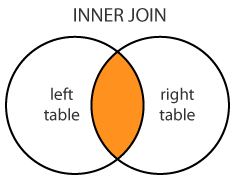
\includegraphics[width=0.3\textwidth]{img/sql-inner-join.png}
    \end{center}
  \end{minipage}
  \caption{Graphical representation of Inner Join}
  \label{inner_join}
\end{figure}

\subsubsection{LEFT JOIN \& RIGHT JOIN}
Left Join returns all of the records in the left table regardless if any of those records have a match in the right table. It will also return all matching records from the right table. Right Join works analogically for the right table\parencite{venn_diagrams}.
\begin{figure}[!ht]
  \centering
  \begin{minipage}{\textwidth}
    \begin{center}
      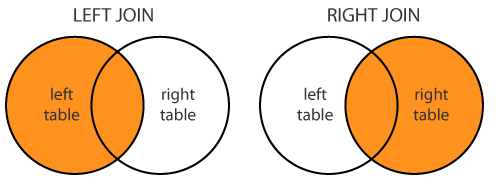
\includegraphics[width=0.6\textwidth]{img/sql-left-right-join.png}
    \end{center}
  \end{minipage}
  \caption{Graphical representation of Left and Right Join}
  \label{lef_right_join}
\end{figure}

The \textit{DataQuery} representation of the join is:
\begin{lstlisting}[language=SQL,escapechar=@,language=SQL,basicstyle=\ttfamily]
SELECT * FROM [LTable] ##JOIN_TYPE## [RTable]
ON [LTable].[LColumn] = [RTable].[RColumn]
\end{lstlisting}


% =============================================================================================
\section{Current implementation}
\label{current implementation}

As described in \autoref{DataQuery concept}, the \textit{DataQuery} currently supports the majority of \textit{SQL} statements. The robustness of the \textit{DataQuery} is also the fact that these statements can also be combined and chained to achieve the desired outcome when both working with in-memory objects and retrieving data from a database. As an example, take the following code:
\begin{lstlisting}
var users = UserInfoProvider.GetUsers()
    .Where("UserName", QueryOperator.Like, "a%", StringComparison.OrdinalIgnoreCase)
    .Where("UserAge", QueryOperator.GreaterOrEquals, 18);
\end{lstlisting}
This chaining will concatenate the \textit{Where} conditions with \textbf{AND} operator, and will return all users whose name starts with \textit{'a'} and their age is greater than or equals to 18.

% ---------------------------------------------------------------------------------------------
\subsection{The Source method}
\label{source method}

The \texttt{Source} method is used to define the source of the query. Its implementation is as follows:
\begin{lstlisting}
public TQuery Source(Action<QuerySource> sourceParameters)
{
    var result = GetTypedQuery();
    // Create source instance from current source
    var source = GetSource();    
    sourceParameters?.Invoke(source);
    result.QuerySource = source;
    
    // Include parameters from source condition
    result.IncludeDataParameters(source.Parameters, source);
    
    return result;
}
\end{lstlisting}


% =============================================================================================
\section{DataQuery insufficiencies}
\label{DataQuery insufficiencies}

Despite these features, the \textit{DataQuery} is not capable of performing the \textit{JOIN} operation in the memory. To join two \textit{Info} objects in Kentico's automated tests, these tests must be of type \textit{integration}. To retrieve the result of joining two \textit{Info} objects, we can use the following code example:
\begin{lstlisting}
var users =
    UserInfoProvider.GetUsers()
        .Source(s =>
            s.Join<UserSettingsInfo>("UserID", "UserSettingsUserID")
        );    
\end{lstlisting}

This will cast the \textit{users} variable to the type \texttt{DataQuery<UserInfo>} which will return \texttt{UserInfo} objects joined on \texttt{UserSettingsInfo} objects where the \texttt{UserID} column of \texttt{UserInfo} object is equal to the \texttt{UserSettingsUserID} column in \texttt{UserSettingsInfo} object. The resulting \textit{SQL} statement:
\begin{lstlisting}[language=SQL,escapechar=@,language=SQL,basicstyle=\ttfamily]
SELECT * FROM [User]
INNER JOIN [UserSettings]
ON [User].[UserID] = [UserSettings].[UserSettingsUserID]
\end{lstlisting}


When invoking the \texttt{Join} lambda function in the \texttt{Source} method, Kentico first processes the object type passed as the \texttt{TObject} type of the \texttt{Join<TObject>(...)} function and only then performs the joining of the two \textit{Info} objects. This processing takes place in the following method:
\begin{lstlisting}
public TSource Join<TObject>
    (string leftColumn, string rightColumn,
     JoinTypeEnum joinType = JoinTypeEnum.Inner,
     IWhereCondition additionalCondition = null)
         where TObject : BaseInfo, new()
{
    return Join(new ObjectSource<TObject>(), leftColumn, rightColumn, additionalCondition, joinType);
}
\end{lstlisting}

Here, the \texttt{new ObjectSource<TObject>()}, the first parameter in the \texttt{return} statement, tries to infer the object source. Firstly, it tries the object type's \texttt{DataSource} property, and secondly, if the \texttt{DataSource} is not defined, it queries the database.

Kentico stores all metadata about its existing classes in the database in the \texttt{CMS\_Class} table. Before finding the object's source, Kentico has to look up the class schema in this table's \texttt{ClassXmlSchema} column in order to know what is the class' schema is and what is the corresponding table name. This table name then becomes the object's source for the automated tests.

When running automated tests inheriting the \texttt{IntegrationTests} class, Kentico sets up a connection string to make database access possible. This has to be an already existing Kentico database with data in contrast with the isolated integration tests. On the other hand, when inheriting the \texttt{UnitTests} base class in our automated tests, this connection string is, naturally, omitted.

Then trying to join two \textit{Info} objects in unit tests fails as the result of the current implementation that does not set correctly the \texttt{DataSource} of the \texttt{TObject}'s type. With the \texttt{DataSource} being \texttt{null} and not having the connection string set up because the inheritance from the \texttt{UnitTests} base class, the \texttt{Join<TObject>()} method fails with a \texttt{NullReferenceExeption} and an error message saying: \texttt{''The ConnectionString property has not been initialized.''}



% =============================================================================================
% TEST AUTOMATION =============================================================================
% =============================================================================================
\chapter{Test automation}
\label{test automation}

In software testing, \textit{test automation} is the use of special software (separate from the software being tested) to control the execution of tests and the comparison of actual outcomes with predicted outcomes. Test automation can automate some repetitive but necessary tasks in a formalized testing process already in place, or perform additional testing that would be difficult to do manually\parencite{test_automation}.

\section{Test automation benefits}
The benefits of test automation are plenty. Below are four common ones:

\begin{compactitem}
    \item \textbf{Reliable} - Tests perform the same operations precisely each time they are run, therefore eliminating human errors.
    \item \textbf{Fast} - Test execution is faster than done manually.
    \item \textbf{Repeatable} - Once tests are created, they can be run repeatedly with little effort, even at lunchtime or after working hours.
    \item \textbf{Regression Testing} - The intent of regression testing is to ensure that a change, such as a bug fix, did not introduce new faults\parencite{test_automation_benefits}.
\end{compactitem}


% =============================================================================================
\section{Unit tests}
\label{unit tests general}

A \textit{unit test} is a piece of a code (usually a method) that invokes another piece of code and checks the correctness of some assumptions afterwards. If the assumptions turn out to be wrong, the unit test has failed. A \textit{unit} is a method or function\parencite{unit_tests}.

A good unit test should:
\begin{compactitem}
  \item be automated and repeatable,
  \item be easy to implement,
  \item run quickly,
  \item be consistent in its results,
  \item have full control of the unit under test,
  \item be fully isolated (runs independently of other tests).
\end{compactitem}

Unit tests are also tests that do not require any external resources, such as a database or network and do not have any external dependencies, such as time or random number generators.


% =============================================================================================
\section{Integration tests}
\label{integration tests general}

\textit{Integration tests} are more complex as they test if different parts of a system are working together correctly and integration testing aims to uncover interaction and compatibility problems as early as possible\parencite{software_testing}.

While working with integration tests, external dependencies such as a database or network access do not necessarily have to be available in the of time the test execution. The biggest issue, however, is the speed. When using unit tests that work with data stored in the memory, the reading speed is high which makes unit tests run admittedly fast. Reading from a database or a remote location on the network introduces a delay in hundreds of milliseconds which might add up to a significant time difference. 
\begin{table}[!ht]
  \begin{tabularx}{\textwidth}{XXX}
    \toprule
     & Unit tests & Integration tests \\
    \midrule
    Speed & \textit{fast} & \textit{slow} \\
    Scope & \textit{narrow}\newline(testing a function or a method) & \textit{wide}\newline(testing different parts of a system) \\
    External\newline dependencies & \textit{no}\newline(using only the memory as data storage) & \textit{yes}\newline(database, network, local disk, ...) \\
    Isolation & \textit{yes}\newline(runs independently of other tests)& \textit{no}\newline(integrates testing of different parts) \\
    Control over\newline the test & \textit{total}\newline(a well written unit test will always run) & \textit{partial}\newline(external resources availability is unknown until the test is executed) \\
    \bottomrule
  \end{tabularx}
  \caption{Comparison of unit and integration tests}
  \label{tab:tests}
\end{table}


% =============================================================================================
\section{Mimicking real objects in automated tests}
\label{mimicking real objects in automated tests}

In general, \textit{Mock} objects are used in software testing to simulate software dependencies so that the testing process can be accelerated and the testing scope can be limited to the component under test (instead of going beyond the interface of dependencies and invoke potential bugs relevant to dependencies).

To simulate real dependencies, mock objects typically have the same interface as the objects they mimic. Therefore, the client object remains unaware of whether it is using a real object or a mock object\parencite{faking_objects}.

In other words, a mock object is simply a testing replacement for a real-world object. A number of situations can come up where mock objects can help us:
\begin{itemize}
    \item The real object is difficult to set up, requiring a certain file system, database, or network environment.
    \item The real object has behaviour that is hard to trigger (for example, a network error).
    \item The real object is slow.
    \item The real object has (or is) a user interface.
    \item The test needs to ask the real object about how it was used (for example, a test might need to confirm that a callback function was actually called).
    \item The real object does not yet exist (a common problem when interfacing with other teams or new hardware systems).
\end{itemize}

Using mock objects, we can get around all of these problems. The three key steps to using mock objects for testing are as follows:
\begin{enumerate}
    \item Use an interface to describe the relevant methods on the object.
    \item Implement the interface for production code.
    \item Implement the interface in a mock object for testing.
\end{enumerate}

The code under test refers to an object only by its interface or base class, so it can remain unaware of whether it is using the real object or the mock\parencite{why_fakes}.

% ---------------------------------------------------------------------------------------------
\subsection{Mocks vs. Fakes vs. Stubs}
\label{mocks vs. fakes vs. stubs}

The term \textit{Mock Objects} has become a popular one to describe special case objects that mimic real objects for testing. Most language environments now have frameworks that make it easy to create mock objects. What's often not realized, however, is that mock objects are but one form of special case test object\parencite{mocks}. Terms used to describe objects that simulate real objects are as follows:
\begin{itemize}
    \item \textbf{Dummy} objects are passed around but never actually used. Usually, they are just used to fill parameter lists.
    \item \textbf{Fake} objects actually have working implementations, but usually, take some shortcut which makes them not suitable for production (an in-memory database is a good example).
    \item \textbf{Stubs} provide canned answers to calls made during the test, usually not responding at all to anything outside what's programmed in for the test.
    \item \textbf{Spies} are stubs that also record some information based on how they were called. One form of this might be an email service that records how many messages it was sent.
    \item \textbf{Mocks} objects pre-programmed with expectations which form a specification of the calls they are expected to receive.
\end{itemize}

Generally, in Kentico, the term \textit{Fake} objects is used to describe \textit{Info} and \textit{InfoProvider} objects that are used in unit tests. Faking objects in Kentico is described in \autoref{faking objects}.



% =============================================================================================
% AUTOMATED TESTING IN KENTICO ================================================================
% =============================================================================================
\chapter{Automated testing in Kentico}
\label{automated testing in Kentico}


% =============================================================================================
\section{Types of tests in Kentico}
\label{kentico tests}

Kentico uses \textit{NUnit} for automated testing. NUnit is an open source unit-testing framework for Microsoft .NET platform and its \textit{assert model} is used in all Kentico's automated tests. More about NUnit framework can be found in \autoref{nunit}.

Kentico's automated tests are divided into three categories: \textit{Unit tests}, \textit{Integration tests}, and \textit{Isolated integration tests}\parencite{kentico_tests}.

% ---------------------------------------------------------------------------------------------
\subsection{Unit tests}
\label{unit tests}

Unit tests are able to run without external resources, such as a database, and execute much faster than the other types of automated tests. When working with \textit{Info} and \textit{InfoProvider} objects, we can avoid accessing the database by using Kentico's fake objects by using \texttt{Fake<TInfo, TInfoProvider>()} method to fake the desired objects. Any unit test containing class must inherit from the \texttt{UnitTests} base class.

% ---------------------------------------------------------------------------------------------
\subsection{Integration tests}
\label{integration test}

Integration tests can access a database provided by a connection string. These tests are used when data read is needed from the database which makes them significantly slower than unit tests. Integration test class inherits the \texttt{IntegrationTests} base class.

% ---------------------------------------------------------------------------------------------
\subsection{Isolated integration tests}
\label{isolated integration test}

Isolated integration tests automatically create their own database before the test execution and clean up the database after the test is finished. This type of tests is the slowest of the three types of automated tests and their base class is \texttt{IsolatedIntegrationTests}.


% =============================================================================================
\section{Faking Info and InfoProvider objects in unit tests}
\label{faking objects}

To create fake data for unit tests, the \texttt{Fake()} method must be called from the \textit{UnitTests} base class (must be inherited by all unit test classes using the \textit{CMS.Tests} library). The method prepares a faked instance of a specific \textit{InfoProvider} class with data. Then use the given InfoProvider's methods to \textit{get}, \textit{create} or \textit{update} data in unit tests.
\begin{lstlisting}
[TestFixture]
public class MyUnitTests : UnitTests
{
    [SetUp]
    public void SetUp()
    {
        // Prepares faked data
        Fake<UserInfo, UserInfoProvider>()
            .WithData(
                new UserInfo
                {
                    UserID = 1,
                    UserName = "FakeUser"
                }
            );
    }

    [Test]
    public void MyTest()
    {
        // Calls a provider method to get user data
        var users = UserInfoProvider.GetUsers();
    }
}
\end{lstlisting}
In the example, \textit{UserInfoProvider} is faked with specific data. Calling \textit{UserInfoProvider} methods to get \textit{UserInfo} objects within tests then returns the faked data instead of accessing the database. The code in the example behaves as if there was a single user named \textit{FakeUser} in the database\parencite{faking_kentico}.

There is \textbf{no need to clean up the faked data before or after running the tests}. Tests inherited from the \textit{UnitTests} base class automatically reset all faked data upon initialization and cleanup.


% =============================================================================================
\section{NUnit framework}
\label{nunit}

\textit{NUnit} is a unit-testing framework for all .NET languages. Initially ported from \textit{JUnit} (unit-testing framework for Java), the current production release, version 3, has been completely rewritten with many new features and support for a wide range of .NET platforms.

% ---------------------------------------------------------------------------------------------
\subsection{Nunit attributes and life cycle}
\label{nunit attributes}

\subsubsection{\texttt{[TestFixture]} attribute} 
This attribute marks a class that contains tests. This attribute can also be used for declaring a base class for other (parametrized) test fixture derived classes to inherit. Test fixtures may take constructor arguments.

\subsubsection{\texttt{[OneTimeSetUp]} and \texttt{[OneTimeTearDown]} attributes} 
These attributes identify methods that are called once prior to and after executing any of the tests in a fixture. If a OneTimeSetUp method fails or throws an exception, none of the tests in the fixture are executed and a failure or error is reported. If any of the methods marked with \textit{OneTimeSetUp} attribute runs, the \textit{OneTimeTearDown} method is guaranteed to run.

\subsubsection{\texttt{[SetUp]} and \texttt{[TearDown]} attributes}
These attributes are used inside a \textit{TestFixture} to provide a common set of functions that are performed just before and just after each test method is called.

Any methods marked with one of the attributes: \texttt{OneTimeSetUp}, \texttt{OneTimeTearDown}, \texttt{SetUp}, or \texttt{TearDown} may be either static or instance methods that can be defined multiple times. Normally, multiple methods are only defined at different levels of an inheritance hierarchy and are run in this order.

\subsubsection{\texttt{[Test]} and \texttt{[TestCase()]} attributes}
The \textit{Test} and \textit{TestCase} attributes are the way of marking a method inside a \textit{TestFixture} class as a test.

The \textit{Test} attribute marks simple (non-parameterized) tests but may also be applied to parameterized tests without causing any extra test cases to be generated.

\textit{TestCase} attribute serves the dual purpose of marking a method with parameters as a test method and providing in-line data to be used when invoking that method.

\subsubsection{\texttt{[TestCaseSource]} attribute}
\textit{TestCaseSource} attribute is used on a parameterized test method to identify the source from which the required arguments will be provided. The attribute additionally identifies the method as a test method. The data is kept separate from the test itself and may be used by multiple test methods.

This attribute can be used in two distinct forms. One to identify the test case data within the same class - usage \texttt{[TestCaseSource(string sourceName)]} or loading the test case data from a different class - usage \texttt{[TestCaseSource(Type sourceType, string sourceName)]}\parencite{nunit_docs}.

% ---------------------------------------------------------------------------------------------
\subsection{Assertions}
\label{assertions}

Assertions are central to unit testing in any of the xUnit frameworks, and NUnit is no exception. NUnit provides a rich set of assertions as static methods of the \texttt{Assert} class.

An assertion method compares the actual value returned by a test to the expected value, and throws an \textit{AssertionException} if the comparison test fails\parencite{assertions}. If a test contains multiple assertions, any that follow the one that failed will not be executed. For this reason, the best practice is one assertion per test.

Each method may be called without a message, with a simple text message or with a message and arguments. In the last case, the message is formatted using the provided text and arguments.

% ---------------------------------------------------------------------------------------------
\subsection{Constraint-based assert Model}
\label{constraint model}

The constraint-based Assert model uses a single method of the \texttt{Assert} class for all assertions. The logic necessary to carry out each assertion is embedded in the constraint object passed as the second parameter to that method.

Using this model, all assertions are made using one of the forms of the \texttt{Assert.That()} method, which has a number of overloads:
\begin{lstlisting}
Assert.That(object actual, IConstraint constraint)
Assert.That(object actual, IConstraint constraint, string message)
Assert.That(object actual, IConstraint constraint, string message, object[] params)

Assert.That(bool condition);
Assert.That(bool condition, string message);
Assert.That(bool condition, string message, object[] parms);
\end{lstlisting}

For overloads taking a constraint, the argument must be an object implementing the \texttt{IConstraint} interface, which supports performing a test on an actual value and generating appropriate messages\parencite{nunit_model}.

Assume there is a method \texttt{GetHypotenuseLength(int a, int b)} that takes two integers as parameters, which represent the legs of a right triangle and calculates the length of the hypotenuse using the Pythagorean theorem. Example of a test case testing this method would look the following:
\begin{lstlisting}
[Test]
public void TestExample()
{
    var length = GetHypotenuseLength(3, 4);
    
    Assert.That(length, Is.EqualTo(5));
}
\end{lstlisting}



% =============================================================================================
% SOLUTION  ===================================================================================
% =============================================================================================
\chapter{Solution and performance measurements}
\label{solution and performance measurements}


% =============================================================================================
\section{Solution}
\label{solution}

To be able to run unit tests containing the \textit{Join} operation on two or more \textit{Info} objects, the following steps need to be undertaken:

\begin{enumerate}
    \item Faking the class structure in unit tests to make sure that the unit tests will not query the database.
    \item Implement logic to the \texttt{Source} method that will prepare the ground to join objects in the memory.
    \item Implement a new layer of abstraction that will have the data sources of both \textit{Info} objects available at the same time.
    \item Implement the logic of joining of the two \textit{Info} objects.
    \item Setting the \texttt{DataSource} property of the query to the result of previously joined objects.
\end{enumerate}

% ---------------------------------------------------------------------------------------------
\subsection{Faking the class structure}
\label{faking the class structure}

In order to avoid querying the database when inferring the object's type (as discussed in \autoref{DataQuery insufficiencies}), the \texttt{DataClassInfo} (code equivalent to the \texttt{CMS\_Class} table) has to be faked in the \texttt{UnitTests} base class. To achieve this the following line of code needs to be added to the \texttt{Init} method in the \texttt{UnitTests} class:
\begin{lstlisting}
[OneTimeSetUp]
public void Init()
{
    Fake<DataClassInfo, DataClassInfoProvider>()
        .WithData();
}
\end{lstlisting}
This will ensure that whenever any piece of code tries to infer an object's type during the run of the tests, it will look into the memory for the faked structure instead of querying the database.

% ---------------------------------------------------------------------------------------------
\subsection{Implementing logic to the \texttt{Source} method}
\label{implementing logic to the Source method}

The \texttt{Source} method (see \autoref{source method}) on the line
\begin{lstlisting}
var source = GetSource();
\end{lstlisting}
gets the \texttt{DataSource} property (\autoref{DataSource}) of the \textit{DataQuery}. If Kentico runs automated unit tests, the type of \texttt{DataSource} is set to \texttt{MemoryDataQuerySource} provided that the \textit{DataQuery} runs in the context of in-memory faked data. We can use this information to create a new layer of abstraction that will allow to join objects in the memory. The following entry is added to the \texttt{Source} method:
\begin{lstlisting}
if (DataSource is MemoryDataQuerySource)
{
    return MemorySource(sourceParameters, result, source);
}
\end{lstlisting}

The \texttt{MemorySource} method is very similar to the \texttt{Source} method but it works with a new memory source that is the new layer of abstraction described in \autoref{new layer of abstraction}. The implementation of the \texttt{MemorySource} method can be found in \autoref{memorysource_method}.


% ---------------------------------------------------------------------------------------------
\subsection{Implementing a new layer of abstraction}
\label{new layer of abstraction}

A new layer of abstraction is needed in order to have the data sources of both objects we are joining available. Since all logic that is required for a successful join takes place in the memory, the new class will be called \texttt{MemorySource} (not to be confused with the method) that will inherit from the \texttt{ObjectSource} class. The key concept of the \texttt{MemorySource} class is that it has three properties:
\begin{itemize}
    \item \texttt{LeftDataSource} that is the data source of the first (or left) object of the join,
    \item \texttt{RightDataSource} that is the data source of the second (or right) object of the join,
    \item \texttt{ResultDataSource} that is the result of the join operation over the left and right objects.
\end{itemize}

The implementation if the \texttt{MemorySource} class can be found in \autoref{memorysource_class}. The \texttt{Join} method in the \texttt{MemorySource} has three key functionalities:
\begin{enumerate}
    \item Setting the \texttt{LeftDataSource} in the constructor,
    \item Setting the \texttt{RightDataSource} and the \texttt{ResultDataSource} in the method \texttt{PrepareDataSources} (see \autoref{preparedatasources}), and
    \item Calling the \texttt{Join} method of the parent class to prepare the correct \texttt{DataQuery}.
\end{enumerate}
   
The \texttt{PrepareDataSources<TObject>} method determines the object source from the \texttt{TObject} generic parameter. As we have already faked the \texttt{DataClassStructure} in \autoref{faking the class structure}, the code will not end with an exception. Next, the code gets the \texttt{InfoProvider} object based on the object source.

Every Kentico's \texttt{InfoProvider} object implements the interface \texttt{ITestableProvider} which contains the \texttt{DataSource} property that is in our case the \texttt{RightDataSource}.

Lastly, the result of the \texttt{InMemoryJoin.Join()} method that handles the logic of the joining of the two data sources is set to the \texttt{ResultDataSource} property of this class which is later assigned to the resulting data source in the \texttt{MemorySource} method.

% ---------------------------------------------------------------------------------------------
\subsection{Implementing the logic of joining}
\label{logic of joining}

Both data sources of the objects to be joined contain the faked data in a \texttt{DataSet}. Each of these datasets contain exactly one \texttt{DataTable} at index \textit{0} and the data rows contained in these tables represent the faked data. One \texttt{DataRow} equals one object created with the \texttt{new} keyword within the \texttt{WithData( new \{ ... \} )} method of the fakes.

\subsubsection{Inner Join}
The logic of joining is done by LINQ and the implementation can be found in \autoref{innerjoin_method}. This method returns all the data rows from both tables that have a match on \texttt{leftRow.Field<int?>(leftColumn)} equals \texttt{rightRow.Field<int?>(rightColumn)} fields.

\subsubsection{Left Join}

This method's implementation can be found in \autoref{leftjoin_method} where the \texttt{GropuJoin} returns every row from the left table with a list of rows from the right table that have a match on the desired columns passed as \texttt{leftColumn} and \texttt{rightColumn} parameters. Furthermore, the \texttt{SelectMany} creates tuples of every left row from the list of matching right rows and combines them into one. The \texttt{DefaultIfEmpty()} method ensures that if the left row has no match in the right table, \texttt{null} will be returned instead of skipping the result.

The right join works in the same manner, only with the difference that it will return every row from the right table with a list of matching rows from the left table\parencite{left_join}.

All of these methods have a reference to the \texttt{CombineDataRows()} method (see \autoref{combinedatarows}). This method takes two data rows and combines them into one. Since no data row can exist without a parent table with its own schema, a new data table is created for the purposes of concatenating the data rows. The resulting data table is a concatenation of the columns of the left and right tables with a simple duplicity check.

% ---------------------------------------------------------------------------------------------
\subsection{Setting the \texttt{DataSource} property}
\label{setting the DataSource}

The previously created data rows that are the result of the join operation are then encapsulated into a new \texttt{DataTable} which is further encapsulated into a new \texttt{DataSet} object that is passed into the constructor of the \texttt{MemoryDataQuerySource}.

This new memory source is then set as the \texttt{ResultDataSource} property of the abstraction described in \autoref{new layer of abstraction}.
\begin{lstlisting}
result.DataSource = memorySource.ResultDataSource;
\end{lstlisting}

The full implementation with all the missing helper methods can be found in the digital appendix to this thesis. The missing methods are omitted from the text as their implementation is not required to understand the context but are absolutely crucial for the final prototype to work correctly.  A brief description how to run the \textit{unit} or \textit{integration} tests can be found in \autoref{digitalcontent}.


% =============================================================================================
\section{Performance measurements}
\label{performance measurements}

Measurement of performance was carried out on the local workstation with parameters:
\begin{itemize}
    \item OS: Windows 7 Enterprise SP1
    \item CPU: Intel(R) Core(TM) i5-4690 (quad core, 6 MB, 3.50 GHz)
    \item RAM: 2 x 8 GB, 1600 MHz, DDR3, Non-ECC
\end{itemize}

Each measurement was performed 10 times in different settings - in memory, using a locally installed database, using a database hosted on a server within Kentico intranet. Using a database hosted on \textit{Microsoft Azure} cloud service was excluded as Kentico does not run its own tests in the cloud.

The measurement was carried out by the \textit{dotTrace}\footnote{https://www.jetbrains.com/profiler/} performance profiler and the measured times are in \textit{milliseconds} with the average being rounded to the nearest whole number. On the next page follow the measurements of the tests.
\newpage

\subsection{Running times of 100 automated tests}
\begin{table}[H]
  \begin{tabularx}{\textwidth}{XXXX}
    \toprule
    Number & Memory & Local DB & Intranet DB \\
    \midrule
    1.  &   818 & 4 715 & 4 130 \\
    2.  & 1 031 & 3 748 & 4 031 \\
    3.  &   709 & 4 160 & 4 229 \\
    4.  &   779 & 3 690 & 4 146 \\
    5.  &   989 & 3 802 & 4 206 \\
    6.  &   828 & 4 193 & 3 978 \\
    7.  & 1 027 & 4 005 & 4 069 \\ 
    8.  &   696 & 4 139 & 4 379 \\
    9.  &   765 & 4 066 & 4 019 \\
    10. &   955 & 4 336 & 3 985 \\
    \bottomrule
    Average & \textbf{860} & \textbf{4 085} & \textbf{4 117} \\
  \end{tabularx}
  \caption{Running times of 100 automated tests in \textit{milliseconds}}
  \label{tab:100tests}
\end{table}

\begin{tikzpicture}
    \begin{axis}
        [enlarge x limits = 0.5,
         ymajorgrids,
         xticklabels = {Memory, Local DB, Intranet DB},
         xtick = {1,...,3},
         ylabel = {Time [ms]},
         width = .9\textwidth]
        \addplot [box plot median] table {100tests.dat};
        \addplot [box plot box] table {100tests.dat};
        \addplot [box plot top whisker] table {100tests.dat};
        \addplot [box plot bottom whisker] table {100tests.dat};
    \end{axis}
\end{tikzpicture}
% ---------------
\subsection{Running times of 500 automated tests}
\begin{table}[H]
  \begin{tabularx}{\textwidth}{XXXX}
    \toprule
    Number & Memory & Local DB & Intranet DB\\
    \midrule
    1.  & 1 072 & 4 317 & 5 330 \\
    2.  &   909 & 4 376 & 5 526 \\
    3.  &   889 & 4 384 & 5 452 \\
    4.  &   856 & 4 282 & 5 214 \\
    5.  &   941 & 4 291 & 5 310 \\
    6.  &   851 & 4 346 & 5 400 \\
    7.  &   957 & 4 355 & 5 089 \\
    8.  &   886 & 4 457 & 5 410 \\
    9.  &   950 & 4 392 & 5 193 \\
    10. &   976 & 4 240 & 5 275 \\
    \bottomrule
    Average & \textbf{929} & \textbf{4 344} & \textbf{5 320}\\
  \end{tabularx}
  \caption{Running times of 500 automated tests in \textit{milliseconds}}
  \label{tab:500tests}
\end{table}

\begin{tikzpicture}
    \begin{axis}
        [enlarge x limits = 0.5,
         ymajorgrids,
         xticklabels = {Memory, Local DB, Intranet DB},
         xtick = {1,...,3},
         ylabel = {Time [ms]},
         width = .9\textwidth]
        \addplot [box plot median] table {500tests.dat};
        \addplot [box plot box] table {500tests.dat};
        \addplot [box plot top whisker] table {500tests.dat};
        \addplot [box plot bottom whisker] table {500tests.dat};
    \end{axis}
\end{tikzpicture}
% ---------------
\subsection{Running times of 1000 automated tests}
\begin{table}[H]
  \begin{tabularx}{\textwidth}{XXXX}
    \toprule
    Number & Memory & Local DB & Intranet DB \\
    \midrule
    1.  & 1 016 & 5 613 & 6 953 \\
    2.  & 1 201 & 4 828 & 7 146 \\
    3.  & 1 113 & 5 364 & 6 809 \\
    4.  & 1 005 & 4 859 & 6 691 \\
    5.  & 1 062 & 4 748 & 7 144 \\
    6.  & 1 236 & 4 934 & 6 900 \\
    7.  & 1 189 & 5 188 & 7 682 \\ 
    8.  & 1 096 & 5 538 & 6 731 \\
    9.  & 1 032 & 4 909 & 7 254 \\
    10. & 1 127 & 4 759 & 6 879 \\
    \bottomrule
    Average & \textbf{1 107} & \textbf{5 074} & \textbf{7 019} \\
  \end{tabularx}
  \caption{Running times of 1000 automated tests in \textit{milliseconds}}
  \label{tab:1000tests}
\end{table}

\begin{tikzpicture}
    \begin{axis}
        [enlarge x limits = 0.5,
         ymajorgrids,
         xticklabels = {Memory, Local DB, Intranet DB},
         xtick = {1,...,3},
         ylabel = {Time [ms]},
         width = .9\textwidth]
        \addplot [box plot median] table {1000tests.dat};
        \addplot [box plot box] table {1000tests.dat};
        \addplot [box plot top whisker] table {1000tests.dat};
        \addplot [box plot bottom whisker] table {1000tests.dat};
    \end{axis}
\end{tikzpicture}

% ---------------------------------------------------------------------------------------------
\subsection{Conclusion}
\label{conclusion}

When using memory as a data storage for the tests instead of a database the performance gain is significant. The automated tests (all types) run after every check-in to Kentico's code base in CI. In addition, these tests are also periodically scheduled to run every night independently of code changes.

\subsubsection{Running 100 tests}
The performance gain of running 100 tests in-memory in comparison with a locally installed database is around \textit{475\%} and around  \textit{479\%} when running tests against a database.

\subsubsection{Running 500 tests}
500 automated tests in-memory gains approximately \textit{468\%} on performance using a local database and \textit{573\%} when having an intranet database.

\subsubsection{Running 1000 tests}
If having 1000 automated tests, the running time improves around \textit{458\%} compared to a locally installed database and \textit{634\%} compared the intranet database.

% ---------------------------------------------------------------------------------------------
\subsection{Testing hidden joins}
Apart from the performance gain, the most significant benefit of this solution is the ability of testing \textit{hidden joins}. This means testing parts of the system implementing the \textit{Join} method without explicitly having to do the necessary joining of objects in the tests.


% =============================================================================================
\section{Extensions and alternative solutions}
\label{extensions and alternative solutions}

% ---------------------------------------------------------------------------------------------
\subsection{Extensions}
\label{extensions}

The current implementation as described in \autoref{logic of joining} joins the objects by fields \texttt{leftColumn} and \texttt{rightColumn} that are passed to the \texttt{Join} method as parameters.

\subsubsection{Supporting other types}

The fields \texttt{leftColumn} and \texttt{rightColumn} are of type \texttt{<int?>} (nullable integer)\parencite{nullable_int} that is the most commonly used type for joins. This implementation can be further extended with generics to support joining on other types, e.g. \texttt{string} is also used every now and then.

\subsubsection{Including a \textit{where} condition}

The \texttt{Join} method can also be extended with one more parameter which would represent a \textit{where} condition to filter out unwanted results right away without adding them to the output and using the \texttt{Where()} method afterwards. The predicate would be represented by a parameter with the type of \texttt{Func<TSource, bool>}. This parameter already resides in the code for easier implementation in the future.

\subsubsection{Leverage multi-threading}

The return type and the type of the first two parameters of the \texttt{Join} method could be changed from \texttt{IEnumerable<DataRow>} to a parallel type \texttt{ParallelQuery<DataRow>} and using the \texttt{AsParallel()} method to run the joining operation in multiple threads using \textit{Parallel LINQ}\parencite{linq}.

\subsubsection{Ordering the results}

When using the \texttt{ParallelQuery<T>} the order of the results is may vary from time to time depending on how many resources has which thread available. To ensure that the result is always in the same order the \texttt{AsOrdered()} method is chained after the \texttt{AsParallel()} method.

% ---------------------------------------------------------------------------------------------
\subsection{Alternative solutions}
\label{alternative solutions}

The only viable alternative solution with the current implementation of the \textit{DataQuery} would be getting all the items of both \textit{Info} objects' data sets through their \texttt{Result} property and perform the join operation on them. Example of such code using the \textit{UserInfo} and \textit{UserSettingsInfo} follows:
\begin{lstlisting}
var users = UserInfoProvider
                .GetUsers().Result;

var userSettings = UserSettingsInfoProvider
                       .GetUserSettings().Result;
                       
var result = Join(users, userSettings, 
                  "UserID", "UserSettingsUserID");
\end{lstlisting}


This solution would still need custom joining logic with the use of LINQ (similar to the current implementation). The resulting \texttt{DataSet} would contain the joined objects but it would lose the \textit{DataQuery} abstraction encapsulating the result.

This effectively means that any other modification of the result would require the use of methods over the \texttt{DataSet} and the containing \texttt{DataTable} or \texttt{DataRow} objects, or additional custom logic that would need further implementation.



% =============================================================================================
% CONCLUSION ==================================================================================
% =============================================================================================
\chapter{Conclusion}

The aim of this thesis was to analyze and extend the current faking of \textit{Info} and \textit{InfoProvider} objects in Kentico's automated tests. The analysis was concluded on Kentico's \textit{DataQuery} API that is an object-oriented abstraction of the database query for reading data.

Chapter three described \textit{DataQuery}, its functionality and a brief listing of methods that make up the \textit{DataQuery}. This chapter also focused on biggest current deficiency which is \textit{DataQuery's} inability to perform \textit{JOIN} operations when inheriting the \texttt{UnitTests} base class, meaning running all operations in the memory.

Chapter five described the types of tests existing in Kentico and further discussed how \textit{faking} of objects in Kentico's automated tests works. Chapter two and four contained theoretical context for chapters three and five respectively.

Chapter six, the most extensive, describes the prototype solution that was used to implement a new layer of abstraction that provides functionality to join two objects in the memory.

This solution enabled to have the data sources of both left and right objects available at the same time and performing the join on them using \textit{LINQ} without losing the \textit{DataQuery} abstraction on the result.

This solution improves on performance as there is no need for a database to perform the joining of the two objects. The performance measurements are available in chapter six as a demonstration of the speed of the tests running in the memory compared to tests running against a database.

Another acquisition of this prototype is allowing of testing methods that in their implementation join two or more objects. In this way, not only explicit joins in the tests can be tested but a whole lot more code containing these \textit{hidden joins}.

Furthermore, chapter six contains also a list of possible future extensions not just to improve the functionality of the implemented join logic but also a suggestion how to further improve the performance using parallelism.

In addition, an alternative solution is briefly discussed in this chapter with stated arguments how it can work and why current prototype is not using this approach.



% =============================================================================================
% BIBLIOGRAPHY ================================================================================
% =============================================================================================
\printbibliography[heading=bibintoc]



% =============================================================================================
% APPENDIX ====================================================================================
% =============================================================================================
\appendix



% =============================================================================================
% IMPLEMENTATIONS =============================================================================
% =============================================================================================
\chapter{Implementations}


% =============================================================================================
\section{MemorySource method}
\label{memorysource_method}

\begin{lstlisting}
/// <summary>
/// Defines a memory source of data.
/// </summary>
private TQuery MemorySource(Action<QuerySource> sourceParameters, TQuery result, QuerySource source)
{
    // Create a new memory source
    var memorySource =
        new MemorySource(DataSource, source);
    
    // Invoke the lambda function
    sourceParameters?.Invoke(memorySource);

    // Set the appropriate sources
    result.QuerySource = memorySource;
    result.DataSource = memorySource.ResultDataSource;

    // Include parameters from source condition
    result.IncludeDataParameters(
    memorySource.Parameters,
        memorySource);

    return result;
}
\end{lstlisting}
\newpage


% =============================================================================================
\section{MemorySource class}
\label{memorysource_class}

\begin{lstlisting}
public class MemorySource : QuerySource
{
    private DataQuerySource LeftDataSource { get; }
    private DataQuerySource RightDataSource;

    public DataQuerySource ResultDataSource;

    public MemorySource(DataQuerySource dataSource, QuerySource querySource)
        : base(querySource)
    {
        LeftDataSource = dataSource;
    }
    
    /// <summary>
    /// Performs a join on the given sources.
    /// </summary>
    public override QuerySource Join<TObject>(
        string leftColumn,
        string rightColumn,
        JoinTypeEnum joinType = JoinTypeEnum.Inner,
        IWhereCondition additionalCondition = null)
    {
        ObjectSource<TObject> objectSource;
    
        // Prepare and set the right and result data source
        PrepareDataSources(out objectSource, leftColumn, rightColumn, additionalCondition, joinType);

        // Encapsulate the result into DataQuery
        return Join(objectSource, leftColumn, rightColumn, additionalCondition, joinType);
    }
}
\end{lstlisting}
\newpage


% =============================================================================================
\section{PrepareDataSources}
\label{preparedatasources}

\begin{lstlisting}
private void PrepareDataSources<TObject>(
    out ObjectSource<TObject> objectSource,
    string leftColumn, string rightColumn,
    WhereCondition additionalCondition = null,
    JoinTypeEnum joinType = JoinTypeEnum.Inner)
            where TObject : BaseInfo, new()
{
    // Create a new object source from <TObject>
    objectSource = new ObjectSource<TObject>();
    objectSource.SourceExpression = GetSourceExpression(new QueryDataParameters());

    // Get the InfoProvider of the right object
    var provider = InfoProviderLoader
                   .GetInfoProvider(
                       objectSource.ObjectType)
                           as ITestableProvider;
    if (provider == null)
    {
        throw new InvalidOperationException($"Info provider for object type '{objectSource.ObjectType}' does not implement '{typeof(ITestableProvider).FullName}'.");
    }

    // Set the right data source
    RightDataSource = provider.DataSource;

    // Join the two data sources
    ResultDataSource = InMemoryJoin.Join(LeftDataSource, RightDataSource, leftColumn, rightColumn, additionalCondition, joinType);
}
\end{lstlisting}
\newpage


% =============================================================================================
\section{Inner join}
\label{innerjoin_method}

\begin{lstlisting}
public IEnumerable<DataRow> Join(
        IEnumerable<DataRow> leftTable,
        IEnumerable<DataRow> rightTable,
        string leftColumn,
        string rightColumn)
{
    return leftTable
    .Join(
        rightTable,
        leftRow =>
            leftRow.Field<int?>(leftColumn),
        rightRow =>
            rightRow.Field<int?>(rightColumn),
        CombineDataRows);
}
\end{lstlisting}
\newpage


% =============================================================================================
\section{Left join}
\label{leftjoin_method}

\begin{lstlisting}
public IEnumerable<DataRow> LeftOuterJoin(
    IEnumerable<DataRow> leftTable,
    IEnumerable<DataRow> rightTable,
    string leftColumn, string rightColumn)
{
    return leftTable.GroupJoin(
        rightTable,
        leftRow =>
            leftRow.Field<int?>(leftColumn),
        rightRow =>
            rightRow.Field<int?>(rightColumn),
        (leftRow, matchingRightRows) => new
        {
            leftRow,
            matchingRightRows
        })
        .SelectMany(
            matchinPairOfRows => matchinPairOfRows.matchingRightRows
                                 .DefaultIfEmpty(),
            (leftRowWithMatchingRightRows, rightRow) =>
            CombineDataRows(
                leftRowWithMatchingRightRows.leftRow,
                rightRow)
        );
}
\end{lstlisting}
\newpage


% =============================================================================================
\section{CombineDataRows}
\label{combinedatarows}
\begin{lstlisting}
public DataRow CombineDataRows(DataRow leftRow, DataRow rightRow)
{
    // Check if the left row has a match
    if (rightRow == null)
    {
        return leftRow;
    }
    
    // Combine the columns from the rows
    var fields = leftRow.ItemArray.Concat(rightRow.ItemArray)
                 .ToArray();
    
    // Create the target table
    var targetTable = CreateTargetTable(
        leftRow.Table,
        rightRow.Table);
    
    // Add the fields to the target table
    targetTable.Rows.Add(fields);
    
    return targetTable.Rows[0];
}
\end{lstlisting}



% =============================================================================================
% DIGITAL CONTENT =============================================================================
% =============================================================================================
\chapter{Digital content}
\label{digitalcontent}

The digital appendix to this thesis (\textit{SLN.zip}) file contains two folders: \textit{SLN\_old} and \textit{SLN\_new}. Both of these contain Kentico's \texttt{Tests} project under name \textbf{CMSTests} and a custom project \textbf{Tests}. To run any of the projects, copy the contents of the folder to a local disk, open the project in \textit{Visual Studio} and build the solution. In both cases, make sure that the restored \textit{NuGet} packages are in the correct version and from the correct source as described in each corresponding section.

% =============================================================================================
\section{SLN\_old}
\label{slnold}

The \textit{SLN\_old} contains a test project called \textbf{Tests} inheriting from the \texttt{UnitTests} to demonstrate the behaviour of the unit tests before the implementation of the solution.

Building this solution should restore the \textit{NuGet} packages \textit{Kentico.Libraries} and \textit{Kentico.Libraries.Dependencies} in version \textit{10.0.0} for the projects and the \textit{NUnit} package in the version \textit{3.2.0} from \textit{nuget.org}\footnote{https://www.nuget.org/}.


% =============================================================================================
\section{SLN\_new}
\label{slnnew}

\textit{SLN\_new} folder's content is similar to the old one, except it contains two extra folders:
\begin{itemize}
    \item \textit{Kentico\_nuget}
    \item \textit{Code\_diff}
\end{itemize}

To ensure the correct run of the tests in this solution, \textbf{it is absolutely vital that the project references the \textit{Kentico.Libraries} and \textit{Kentico.Libraries.Dependencies} in the version \textit{11.0.0-B1709081005-2341} from the \textit{Kentico\_nuget} folder} and NUnit \textit{3.9.0} from \textit{nuget.org}. \textbf{When managing the NuGet packages for this solution, the \textit{Include prerelease} option must be checked in \textit{Visual Studio}.}

The \textit{Code\_diff} folder contains independent \texttt{.cs} files and screenshots with all the changes in code from the solution including all the helper methods omitted from \autoref{solution and performance measurements}.


% =============================================================================================
\section{Running integration tests in Kentico}
\label{runningintegrationtests}

To run integration tests in Kentico, a database with data is required. Obtaining Kentico with a database with sample data can be achieved by downloading Kentico from the official web page and installing on the local machine.

Downloading Kentico from \textit{https://www.kentico.com/download-demo/} will let the user choose from either a free license or a trial version. Creating an integration test after the installation can be done in just a few minutes by taking the following steps:
\begin{enumerate}
    \item Create a \textit{Tests} project.
    \item Create an integration test (the code from \textit{SLN\_new} can be used).
\end{enumerate}

Both steps are described in Kentico's official documentation on the following pages:
\begin{enumerate}
    \item Creating a tests project:\newline
    \textit{https://docs.kentico.com/k10/custom-development/writing-automated-tests/creating-automated-test-projects}
    \item Creating an integration test:\newline
    \textit{https://docs.kentico.com/k10/custom-development/writing-automated-tests/creating-integration-tests-with-a-connection-string}
\end{enumerate}


\end{document}